\documentclass[xcolor={dvipsnames},pdf, hyperref={colorlinks=true, citecolor=ForestGreen, linkcolor=BlueViolet, urlcolor=Magenta}]{beamer}
\usetheme{Frankfurt}  
\usecolortheme{whale}
\usepackage{tikz} 
\usepackage{amsmath}
\usepackage{amsthm}
\usepackage{amssymb}              % used for \eqref{} in this document
\usepackage{dsfont}
\usepackage{hyperref}
\usepackage{threeparttable}
\usepackage{multirow}
\graphicspath{{Figures/}}
\usepackage{booktabs}
\usepackage{tikz}
\newtheorem{exmp}{Example}[section]
\usepackage{subcaption}
\usepackage{adjustbox}
\usepackage{graphicx}
\usepackage[mathscr]{euscript}
\usepackage{remreset}% tiny package containing just the \@removefromreset command
\makeatletter
\@removefromreset{subsection}{section}
\makeatother
\setcounter{subsection}{1}
\usepackage{float}
\usepackage{sgamevar}
\usepackage{sgame}
\theoremstyle{definition}


\newcommand{\defn}[1]{\textbf{#1}}


%Instructor version
\newcommand{\blank}[0]{}
\newcommand{\ddp}[1]{{\textcolor{ForestGreen}{#1}}} 
\newcommand{\dd}[1]{{\underline{\textcolor{ForestGreen}{#1}}}}

%Student version
%\newcommand{\blank}[0]{\vspace{2em}}
%\newcommand{\dd}[1]{\underline{\hspace{3cm}}} 
%\newcommand{\ddp}[1]{}

\addtobeamertemplate{navigation symbols}{}{%
	\usebeamerfont{footline}%
	\usebeamercolor[fg]{footline}%
	\hspace{1em}%
	\insertframenumber/\inserttotalframenumber
}

\section{Absolute Advantage}

%% preamble
\title{Interdependence and the Gains from Trade}
\author{David A. D\'iaz}
\institute{UNC Chapel Hill}
\date{}

\AtBeginSection[] %Section links on slides

\begin{document} 
	
	\begin{frame}
		
		\titlepage
		
	\end{frame}
	
\begin{frame}{Trade}
	\begin{itemize}
		\item \textbf{Principle 5: Trade Can Make Everyone Better Off}
		\item Trade allows countries (or people) to specialize in what they do best and enjoy a greater variety of good and services.
	\end{itemize}
\end{frame}

\begin{frame}{Ratios and Unit Conversion}
	\begin{exmp}
	\begin{enumerate}
		\item 	Express the ratio $25$ apples $: 75$ oranges in three different ways. 
		\item Josh takes 12 hours to produce 25 coconuts. How many coconuts can he produce in one day? In one week? \\
	\end{enumerate}
	\end{exmp}
	\pause \ddp{(1) $1a : 3o$, $1/3a : 1o$, $50a : 150o$, etc. \\
	(2) 25 coconuts/12 hours $\times$ 24 hours/day = 50 coconuts/day. 50 coconuts/day $\times$ 7 days/week = 350/week.}
\end{frame}

\begin{frame}{Ratios and Unit Conversion}
	\begin{exmp} 
	Instead of coconuts, Josh can use his time to produce pineapples. In 12 hours, he can produce 5 pineapples. If he uses his whole day to produce coconuts, how many pineapples is he giving up? What is his opportunity cost of producing one coconut?
\end{exmp}
\pause \ddp{5 pineapples/12 hours $\times$ 24 hours/day = 10 pineapples/day. \\
	He gives up 10 pineapples to produce 50 coconuts. 
	\\ Ratio: 10 pineapples : 50 coconuts $\Rightarrow$ 1 coconut : 1/5 pineapple. OC of 1 coconut is 1/5 a pineapple.}
\end{frame}


\begin{frame}{Absolute Advantage}
	
	\begin{itemize}
	\item 	\defn{Absolute Advantage:} 
	\begin{enumerate}
			\item The ability to produce a good using fewer inputs than another producer.
			\item The ability to produce more units of a good using the same number of inputs.
		\end{enumerate}
	\end{itemize}
	
	\begin{exmp}
		Pepe can grow 25 potatoes in one day, while Silvia can grow 20 potatoes in a day. Who has an absolute advantage in the production of potatoes? Why?
	\end{exmp} 
	\pause \ddp{Pepe has AA because he can produce more potatoes than Silvia using the same number of inputs (1 day).}
\end{frame}




\begin{frame}[t]{Absolute Advantage}
		\begin{exmp} 
			The following table shows the production possibilities available to Harold and Kumar:
			
			\begin{table}[H]
				\caption*{Minutes needed to make 1 ounce of:}
				\centering
				\begin{tabular}{c|c|c|}
					
					& Beans & Porridge \\
					\hline
					Harold & 20 min/oz & 15 min/oz \\
					
					Kumar  & 30 min/oz & 60 min/oz \\
					
				\end{tabular}
			\end{table}
			
			Who has an absolute advantage in the production of beans? Of porridge? Why?
		\end{exmp}
		
	\pause 	\ddp{Harold has an AA in both goods because she can produce 1 oz of each good using fewer inputs than Kumar.}
		
	\end{frame}


\section{Comparative Advantage}


\begin{frame}{Comparative Advantage}
	\begin{itemize}
		\item 	\defn{Comparative Advantage:} The ability to produce a good at a lower opportunity cost than another producer.
		
		\begin{exmp}
			Instead of potatoes, Pepe \& Silvia could produce yuccas. Pepe can grow 50 yuccas in a day and Silvia can grow 80. What is the opportunity cost of 1 potato for Pepe? For Silvia? Who has the comparative advantage in the production of potatoes?
		
		\end{exmp} 
		
	\pause 	\ddp{Pepe: 25 P : 50 Y $\Rightarrow$ 1 P : 2 Y; 1 Y : 1/2 P.\\
			Silvia: 20 P : 80 Y $\Rightarrow$ 1 P : 4 Y; 1 Y : 1/4 P. \\
			Pepe has the CA in potatoes, Silvia has the CA in yuccas.}
	\end{itemize}
	\end{frame}
	
\begin{frame}[t]{Comparative Advantage}
		\begin{exmp}
			What is the opportunity cost of 1 ounce of beans for Harold? For Kumar? What is the opportunity cost of 1 ounce of porridge for each? Who has the comparative advantage in each good?
		\end{exmp} 
		\ddp{\pause Harold: \\
		20 min/1 oz beans : 15 min/1 oz porridge \\
		\pause $\Rightarrow$ 1 oz beans/20 min : 1 oz porridge/15 min \\
		\pause $\Rightarrow$ 1 oz beans : 1.33 oz of porridge; 1 oz porridge : .75 oz beans. \\ 
		\pause Kumar: \\
		30 min/1 oz beans : 60 min/1 oz porridge \\
		 \pause $\Rightarrow$ 1 oz beans/30 min : 1 oz porridge/60 min \\
		 \pause $\Rightarrow$ 1 oz beans : 1/2 oz of porridge, 1 oz porridge : 2 oz beans. \\
		\pause	Kumar has the CA in beans, Harold has the CA in porridge.}
\end{frame}
	
\begin{frame}{Comparative Advantage}
	\begin{itemize}
		\item 	It is possible for one person to have an absolute advantage in both goods. 
		\item Not possible to have a comparative advantage in both goods. Why? 
			\begin{itemize}
				\item The opportunity cost of one good is the \dd{reciprocal} of the other. If the opportunity cost of one good is relatively high, the opportunity cost of the other good must be relatively low.
			\end{itemize} 
	\item	\textbf{Unless the two parties have the same opportunity costs, one person will have a comparative advantage in one good, and the other party will have a comparative advantage in the other good.}
	\end{itemize}
\end{frame}
	
		\begin{frame}[t]{Comparative Advantage}
			
			\begin{exmp}
				\scriptsize
			Refer to Table \ref{tab1}, which shows the combinations of cheese and wine that Italy and France can produce in a day.
			\begin{table}[H]
				\caption{Production in Italy \& France}
				\label{tab1}
				\centering
				\begin{tabular}{ cccc} 
					
					\multicolumn{2}{c}{\underline{Italy}} &  \multicolumn{2}{c}{\underline{France}}  \\
					\underline{Wine (bottles)} & \underline{Cheese (lbs)}  & \underline{Wine (bottles)} & \underline{Cheese (lbs)}  \\
				
					0 & 8 & 0 & 15 \\
					1 & 6 & 1 & 12 \\
					2 & 4 & 2 & 9\\
					3 & 2 & 3 & 6 \\
					4 & 0 & 4 & 3 \\
					&& 5 & 0 \\
				\end{tabular}
			\end{table}	
			Who was the comparative advantage in producing each good?
			\end{exmp}
		\scriptsize
	\pause	\ddp{Italy: 1 bottle wine: 2 lbs cheese. France: 1 bottle wine: 3 lbs cheese $\Rightarrow$ Italy has CA in producing wine. France has CA in producing cheese.}	
		\end{frame}
	
\begin{frame}{The Gains from Trade}
	
		\begin{itemize}
			
			\item 	The gains from trade are based on \dd{comparative advantage}. 
				\begin{itemize}
					\item When each party specializes in producing the good for which they have a  \dd{lower opportunity cots}, total production in the economy increases. 
				\end{itemize}
			\item 	To illustrate this, let's use the example with Pepe and Silvia.
			
			\begin{table}[H]
				\caption*{Daily production of potatoes and yucca:}
				\centering
				\begin{tabular}{ c|c|c|}        
					
					& Potatoes & Yuccas \\
					\hline
					Pepe & 25 & 50  \\
					
					Silvia  & 20 & 80  \\
					
				\end{tabular}
			\end{table}
		\end{itemize}

\section{The Gains from Trade}
	
\end{frame}


\begin{frame}{The Gains from Trade}
	
\begin{itemize}
	\item Suppose that currently, Pepe produces and consumes 15 potatoes and 20 yuccas
	\item Silvia produces and consumes 10 potatoes and 40 yuccas
	\item Thus, between them, they are currently producing 25 potatoes and 60 yuccas.

\end{itemize}
		
\end{frame}

\begin{frame}{The Gains from Trade}
	
\begin{itemize}
	\item 	Pepe has a comparative advantage in potatoes and Silvia has a comparative advantage in yuccas. 
	\item Therefore with trade, Pepe will export \dd{potatoes} to Silvia and import \dd{yuccas}. 
	\item Suppose that Pepe and Silvia decide to exchange at a rate of 1 potato for 3 yuccas. This is their so-called \dd{``terms of trade''}.
	\item What happens to their production and consumption if they decide trade 10 potatoes for yuccas? Note: Always assume complete specialization.
\end{itemize}
	
\end{frame}

\begin{frame}{The Gains from Trade}
	\begin{itemize}
		\item Pepe: Produces 25 potatoes and exports 10 in exchange for 30 yuccas. Did his consumption of potatoes and yuccas increase vs. autarky?
		\item Silvia: Produces 80 yuccas and exports 30 in exchange for 10 potatoes. Did his consumption of potatoes and yuccas increase vs. autarky?
		
		
		\item Pepe  and Silvia can now consume at points which were impossible without trade. 
		\item Total production in the economy is now 25 potatoes and 80 yuccas, so total production increased as well.
		\item \textbf{Comparative advantage and specialization allow for increased consumption by \textbf{both} parties and increased total production in the economy.}
	\end{itemize}
\end{frame}

\begin{frame}[b]{The Gains from Trade}
	\begin{figure}[HB]
			\ddp{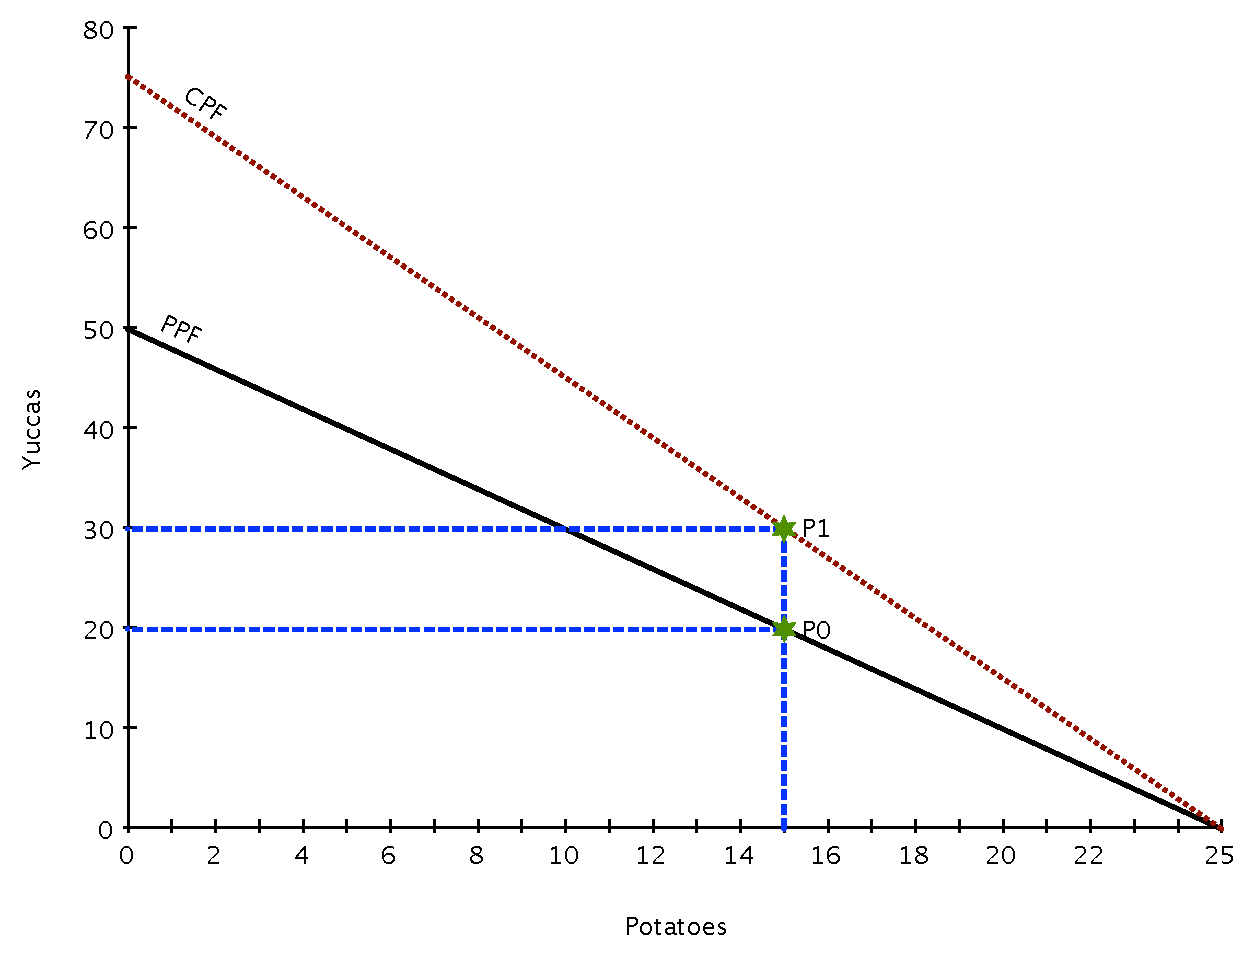
\includegraphics[scale=.35]{plot5.pdf}}
			\caption{Pepe's PPF \& CPF}
		\end{figure}
\end{frame}

\begin{frame}[b]{The Gains from Trade}
	\begin{figure}[HB]
		\ddp{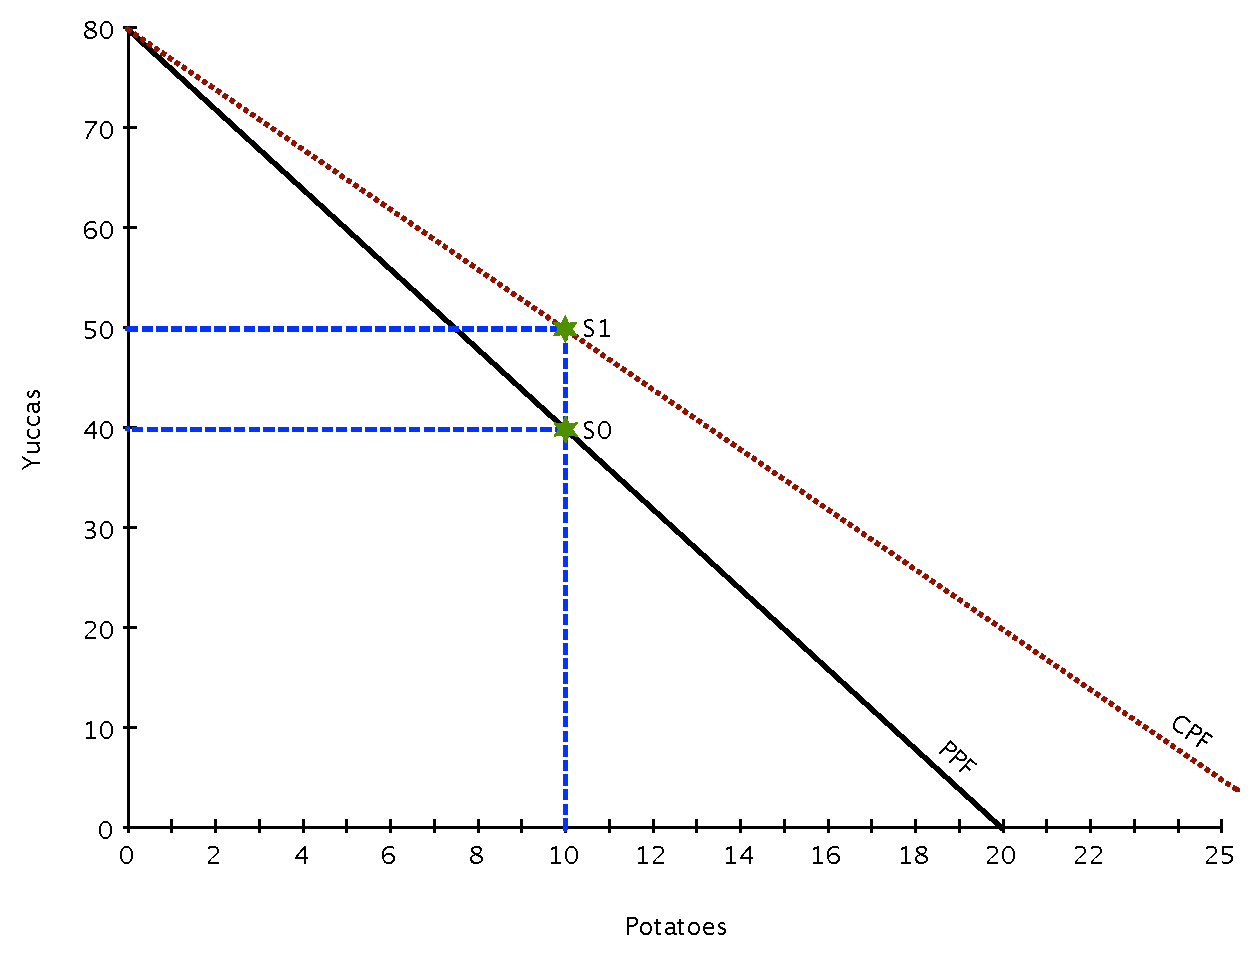
\includegraphics[scale=.35]{plot6.pdf}}
		\caption{Silvia's PPF \& CPF}
	\end{figure}
\end{frame}


\begin{frame}{Setting the Price of Trade}
	
	\begin{itemize}
		\item In order for trade to be beneficial, it must make both parties better off. 
		\item In order to do so, the terms of trade must lie between the \dd{opportunity costs} of each party. 
		\item Consider Pepe and Silvia's trade from the perspective of each party in terms of potatoes.
	\end{itemize}
	
\end{frame}

\begin{frame}{Setting the Price of Trade}
	\begin{itemize}
		\item \textit{Pepe's perspective}:
			\begin{itemize}
				\item Exports potatoes in exchange for yuccas.
				\item On his own, Pepe gives up 2 yuccas for each potato.
				\item Thus, he is only better off if he receives \underline{more} than 2 yuccas for each potato he exports.
			\end{itemize}
	\end{itemize}
\end{frame}

\begin{frame}{Setting the Price of Trade}
\begin{itemize}
		\item \textit{Silvia's perspective:}
		\begin{itemize}
			\item Imports potatoes in exchange for yuccas.
			\item On his own, Silvia gives up 4 yuccas for each potato.
			\item Thus, he is only better off if he gives up \underline{less} than 4 yuccas for each potato he imports.
		\end{itemize}  
		
		\item Thus, if expressing the terms of trade as 1 potato $: X$ yuccas, it has to be that 2 $< X <$ 4 in order for both parties to be better off.
	\end{itemize}
\end{frame}

\begin{frame}[t]{Setting the Price of Trade}
	\begin{exmp}
		\scriptsize
		The table below shows the output per person per day in the US and Japan, who make either drugs or TVs. Assume worker skills are not specialized. 
		
		\begin{table}
			\begin{tabular}{c| c |c }
				& Drugs & TVs  \\
				\hline 
				US & 16 & 32 \\ 
				Japan & 8 & 24 \\
			\end{tabular}
		\end{table}
	\begin{enumerate}
		\item Which country has the absolute advantage in producing drugs? In producing TVs?
		\item What is the opportunity cost of producing one TV in each country?
		\item What is the opportunity cost of producing one drug in each country?
		\item If the countries decide to trade, what will be the trade pattern?
	\end{enumerate}
	\end{exmp}
	\scriptsize
\ddp{\pause 1. The US has the AA in producing both goods.\\
	\pause	2. US: 1 TV : 1/2 drug. Japan: 1 TV : 1/3 drug. \\
	\pause	3. US: 1 drug : 2 TVS. Japan: 1 drug: 3 TVs. \\
	\pause	4. US has CA in drugs, Japan has CA in TVs. US exports drugs for TVs.}
\end{frame}

\begin{frame}[t]{Setting the Price of Trade}
	\begin{exmp}
		\scriptsize
		Suppose the following terms of trade are proposed:	 
		 \begin{enumerate}[(i)]
			\item 10 TVs : 20 drugs
			\item 45 TVs: 180 drugs
			\item 50 TVs: 300 drugs
			\item 60 TVs : 10 drugs 	
		\end{enumerate}
	\begin{enumerate}
		\item Which of the terms of trade are acceptable to Japan, but not to the US?
		\item Which of the terms of trade are acceptable to the US, but not to Japan?
		\item Come up with 3 terms of trade that would be acceptable to both parties.
	\end{enumerate} 
	\end{exmp}
	\scriptsize
	\ddp{\pause Terms of trade: 1 drug : $X$ TVs. If $X<2$, US worse off. If $X>3$, Japan worse off. \\
		\pause  (i) 1 drug : 1/2 TV $\Rightarrow$ US worse off.  (ii) 1 drug : 1/4 TV $\Rightarrow$ US worse off. \\
	 (iii) 1 drug : 1/6 TV $\Rightarrow$ US worse off. (iv) 1 drug : 6 TVs $\Rightarrow$ Japan worse off. \\
	\pause	Acceptable: 1 drug : 2.5 TVs, 10 drugs : 25 TVs, 40 drugs : 100 TVs}
\end{frame}

\begin{frame}{Readings and Assignments}
	\begin{itemize}
		\item Today: Mankiw Ch. 3
		\item Next time: Mankiw Ch. 4
		\item Problem Set 1, section 2
	\end{itemize}

\end{frame}

\end{document}